% Options for packages loaded elsewhere
\PassOptionsToPackage{unicode}{hyperref}
\PassOptionsToPackage{hyphens}{url}
%
\documentclass[
  a4paper,
]{article}
\usepackage{amsmath,amssymb}
\usepackage{iftex}
\ifPDFTeX
  \usepackage[T1]{fontenc}
  \usepackage[utf8]{inputenc}
  \usepackage{textcomp} % provide euro and other symbols
\else % if luatex or xetex
  \usepackage{unicode-math} % this also loads fontspec
  \defaultfontfeatures{Scale=MatchLowercase}
  \defaultfontfeatures[\rmfamily]{Ligatures=TeX,Scale=1}
\fi
\usepackage{lmodern}
\ifPDFTeX\else
  % xetex/luatex font selection
  \setmainfont[]{Helvetica}
\fi
% Use upquote if available, for straight quotes in verbatim environments
\IfFileExists{upquote.sty}{\usepackage{upquote}}{}
\IfFileExists{microtype.sty}{% use microtype if available
  \usepackage[]{microtype}
  \UseMicrotypeSet[protrusion]{basicmath} % disable protrusion for tt fonts
}{}
\makeatletter
\@ifundefined{KOMAClassName}{% if non-KOMA class
  \IfFileExists{parskip.sty}{%
    \usepackage{parskip}
  }{% else
    \setlength{\parindent}{0pt}
    \setlength{\parskip}{6pt plus 2pt minus 1pt}}
}{% if KOMA class
  \KOMAoptions{parskip=half}}
\makeatother
\usepackage{xcolor}
\usepackage[margin=1in]{geometry}
\usepackage{graphicx}
\makeatletter
\def\maxwidth{\ifdim\Gin@nat@width>\linewidth\linewidth\else\Gin@nat@width\fi}
\def\maxheight{\ifdim\Gin@nat@height>\textheight\textheight\else\Gin@nat@height\fi}
\makeatother
% Scale images if necessary, so that they will not overflow the page
% margins by default, and it is still possible to overwrite the defaults
% using explicit options in \includegraphics[width, height, ...]{}
\setkeys{Gin}{width=\maxwidth,height=\maxheight,keepaspectratio}
% Set default figure placement to htbp
\makeatletter
\def\fps@figure{htbp}
\makeatother
\setlength{\emergencystretch}{3em} % prevent overfull lines
\providecommand{\tightlist}{%
  \setlength{\itemsep}{0pt}\setlength{\parskip}{0pt}}
\setcounter{secnumdepth}{-\maxdimen} % remove section numbering
\usepackage{titling}
\pretitle{\begin{flushleft}}
\posttitle{\end{flushleft}}
\usepackage{booktabs}
\usepackage{longtable}
\usepackage{float}
\usepackage{colortbl}
\usepackage{pdflscape}
\usepackage{tabu}
\usepackage{makecell}
\usepackage{xcolor}
\usepackage{soul}
\usepackage{caption}
\usepackage[singlelinecheck=false]{caption}
\usepackage[font={footnotesize,it}]{caption}
\usepackage{booktabs}
\usepackage{longtable}
\usepackage{array}
\usepackage{multirow}
\usepackage{wrapfig}
\usepackage{float}
\usepackage{colortbl}
\usepackage{pdflscape}
\usepackage{tabu}
\usepackage{threeparttable}
\usepackage{threeparttablex}
\usepackage[normalem]{ulem}
\usepackage{makecell}
\usepackage{xcolor}
\ifLuaTeX
  \usepackage{selnolig}  % disable illegal ligatures
\fi
\usepackage{bookmark}
\IfFileExists{xurl.sty}{\usepackage{xurl}}{} % add URL line breaks if available
\urlstyle{same}
\hypersetup{
  hidelinks,
  pdfcreator={LaTeX via pandoc}}

\title{\vspace{-1.5cm} \begin{LARGE} WGS Quality Control Report \end{LARGE}}
\author{}
\date{\vspace{-2.5em}}

\begin{document}
\maketitle

\normalsize Batch Name: 2024-05-03

\normalsize Experiment Name: 24ARS\_STC\_TRIC\_LG733

\fontsize{7}{8}
\selectfont
\captionsetup[table]{labelformat=empty}
\renewcommand{\arraystretch}{1.2}

\begin{longtable}[t]{>{\centering\arraybackslash}p{1cm}>{\centering\arraybackslash}p{2cm}>{\centering\arraybackslash}p{1.5cm}>{\centering\arraybackslash}p{5.25cm}>{\centering\arraybackslash}p{5.25cm}}
\toprule
\multicolumn{1}{>{\centering\arraybackslash}p{1cm}}{\cellcolor[HTML]{D4D4D4}{\textbf{Isolate No.}}} & \multicolumn{1}{>{\centering\arraybackslash}p{2cm}}{\cellcolor[HTML]{D4D4D4}{\textbf{Sample ID}}} & \multicolumn{1}{>{\centering\arraybackslash}p{1.5cm}}{\cellcolor[HTML]{D4D4D4}{\textbf{Description}}} & \multicolumn{1}{>{\centering\arraybackslash}p{5.25cm}}{\cellcolor[HTML]{D4D4D4}{\textbf{ARSRL}}} & \multicolumn{1}{>{\centering\arraybackslash}p{5.25cm}}{\cellcolor[HTML]{D4D4D4}{\textbf{WGS}}}\\
\midrule
1 & 23ARS\_BGH0073 & EMR100 & Klebsiella pneumoniae & \cellcolor{white}{Klebsiella pneumoniae}\\
2 & 23ARS\_DMC0672 & EMR132 & Klebsiella pneumoniae & \cellcolor{white}{Klebsiella pneumoniae}\\
3 & 24ARS\_BRT0006 & EMR137 & Klebsiella pneumoniae & \cellcolor{white}{Klebsiella pneumoniae}\\
4 & 24ARS\_BRT0009 & EMR138 & Klebsiella pneumoniae & \cellcolor{white}{Klebsiella quasipneumoniae}\\
5 & 24ARS\_BRT0011 & EMR139 & Klebsiella pneumoniae & \cellcolor{white}{Klebsiella pneumoniae}\\
\addlinespace
6 & 24ARS\_BRT0016 & EMR140 & Pseudomonas aeruginosa & \cellcolor{white}{Pseudomonas aeruginosa}\\
7 & 24ARS\_EVR0004 & EMR135 & Escherichia coli & \cellcolor{white}{Escherichia coli}\\
8 & 24ARS\_STC\_CVM001 & satscan & Escherichia coli & \cellcolor{white}{Escherichia coli}\\
9 & 24ARS\_STC\_CVM002 & satscan & Klebsiella pneumoniae & \cellcolor{white}{Klebsiella pneumoniae}\\
10 & 24ARS\_STC\_CVM003 & satscan & Escherichia coli & \cellcolor{white}{Escherichia coli}\\
\addlinespace
11 & 24ARS\_STC\_CVM004 & satscan & Escherichia coli & \cellcolor{white}{Escherichia coli}\\
12 & 24ARS\_STC\_CVM005 & satscan & Escherichia coli & \cellcolor{white}{Escherichia coli}\\
13 & 24ARS\_STC\_CVM006 & satscan & Klebsiella pneumoniae & \cellcolor{white}{Klebsiella pneumoniae}\\
14 & 24ARS\_STC\_CVM007 & satscan & Klebsiella pneumoniae & \cellcolor{white}{Klebsiella pneumoniae}\\
15 & 24ARS\_STC\_CVM008 & satscan & Klebsiella pneumoniae & \cellcolor{white}{Klebsiella quasipneumoniae}\\
\addlinespace
16 & 24ARS\_STC\_CVM009 & satscan & Klebsiella pneumoniae & \cellcolor{white}{Klebsiella pneumoniae}\\
17 & UTP\_BL\_007 & tricycle & Escherichia coli & \cellcolor{white}{Escherichia coli}\\
18 & UTP\_BL\_008 & tricycle & Escherichia coli & \cellcolor{white}{Escherichia coli}\\
19 & UTP\_BL\_009 & tricycle & Escherichia coli & \cellcolor{white}{Escherichia coli}\\
20 & UTP\_BL\_010 & tricycle & Escherichia coli & \cellcolor{white}{Escherichia coli}\\
\addlinespace
21 & UTP\_BL\_011 & tricycle & Escherichia coli & \cellcolor{white}{Escherichia coli}\\
22 & UTP\_ST\_055 & tricycle & Escherichia coli & \cellcolor{white}{Escherichia coli}\\
\bottomrule
\end{longtable}

\tiny Legend: \begingroup\fontsize{4}{6}\selectfont

\begin{tabular}{|>{\centering\arraybackslash}p{1cm}|>{\centering\arraybackslash}p{1cm}|>{\centering\arraybackslash}p{1cm}|>{\centering\arraybackslash}p{3cm}|>{\centering\arraybackslash}p{2cm}|}

\cellcolor{white}{PASS} & \cellcolor[HTML]{FFA77F}{WARNING} & \cellcolor[HTML]{FD7979}{FAILURE} & \textcolor{blue}{EXCEEDS THRESHOLD METRIC/S} & \cellcolor{yellow}{NON-CONCORDANT}\\

\end{tabular}
\endgroup{}
\fontsize{7}{8}
\selectfont
\captionsetup[table]{labelformat=empty}
\renewcommand{\arraystretch}{1.2}

\(\\\)

\fontsize{7}{8}
\selectfont
\captionsetup[table]{labelformat=empty}
\renewcommand{\arraystretch}{1.2}

\begin{longtable}[t]{>{\centering\arraybackslash}p{1cm}>{\centering\arraybackslash}p{3cm}>{\centering\arraybackslash}p{2cm}>{\centering\arraybackslash}p{2cm}>{\centering\arraybackslash}p{2cm}>{\centering\arraybackslash}p{2cm}>{\centering\arraybackslash}p{2cm}}
\toprule
\multicolumn{1}{>{\centering\arraybackslash}p{1cm}}{\cellcolor[HTML]{D4D4D4}{\textbf{Isolate No.}}} & \multicolumn{1}{>{\centering\arraybackslash}p{3cm}}{\cellcolor[HTML]{D4D4D4}{\textbf{Sample ID}}} & \multicolumn{1}{>{\centering\arraybackslash}p{2cm}}{\cellcolor[HTML]{D4D4D4}{\textbf{Contamination}}} & \multicolumn{1}{>{\centering\arraybackslash}p{2cm}}{\cellcolor[HTML]{D4D4D4}{\textbf{Contigs}}} & \multicolumn{1}{>{\centering\arraybackslash}p{2cm}}{\cellcolor[HTML]{D4D4D4}{\textbf{GC Percent}}} & \multicolumn{1}{>{\centering\arraybackslash}p{2cm}}{\cellcolor[HTML]{D4D4D4}{\textbf{N50}}} & \multicolumn{1}{>{\centering\arraybackslash}p{2cm}}{\cellcolor[HTML]{D4D4D4}{\textbf{Total Length}}}\\
\midrule
1 & 23ARS\_BGH0073 & \textcolor{black}{0} & \textcolor{black}{77} & 56.70 & \textcolor{black}{245773} & 5784839\\
2 & 23ARS\_DMC0672 & \textcolor{black}{0} & \textcolor{black}{107} & 57.14 & \textcolor{black}{322650} & 5641788\\
3 & 24ARS\_BRT0006 & \textcolor{black}{0} & \textcolor{black}{71} & 57.14 & \textcolor{black}{266742} & 5591154\\
4 & 24ARS\_BRT0009 & \textcolor{black}{0} & \textcolor{black}{59} & 57.67 & \textcolor{black}{290040} & 5446056\\
5 & 24ARS\_BRT0011 & \textcolor{black}{0} & \textcolor{black}{95} & 57.04 & \textcolor{black}{196758} & 5711812\\
\addlinespace
6 & 24ARS\_BRT0016 & \textcolor{black}{0} & \textcolor{black}{117} & 66.02 & \textcolor{black}{181908} & 6802621\\
7 & 24ARS\_EVR0004 & \textcolor{black}{0} & \textcolor{black}{53} & 50.48 & \textcolor{black}{340285} & 5067237\\
8 & 24ARS\_STC\_CVM001 & \textcolor{black}{0} & \textcolor{black}{64} & 50.70 & \textcolor{black}{236861} & 4782190\\
9 & 24ARS\_STC\_CVM002 & \textcolor{black}{0} & \textcolor{black}{23} & 57.46 & \textcolor{black}{471275} & 5307898\\
10 & 24ARS\_STC\_CVM003 & \textcolor{black}{0} & \textcolor{black}{86} & 50.51 & \textcolor{black}{130631} & 4709613\\
\addlinespace
11 & 24ARS\_STC\_CVM004 & \textcolor{black}{0} & \textcolor{black}{72} & 50.80 & \textcolor{black}{127236} & 4660175\\
12 & 24ARS\_STC\_CVM005 & \textcolor{black}{0} & \textcolor{black}{125} & 50.90 & \textcolor{black}{90736} & 4711453\\
13 & 24ARS\_STC\_CVM006 & \textcolor{black}{0} & \textcolor{black}{51} & 57.01 & \textcolor{black}{392911} & 5498661\\
14 & 24ARS\_STC\_CVM007 & \textcolor{black}{0} & \textcolor{black}{87} & 56.94 & \textcolor{black}{338934} & 5549988\\
15 & 24ARS\_STC\_CVM008 & \textcolor{black}{0} & \textcolor{black}{20} & 57.85 & \textcolor{black}{929710} & 5214271\\
\addlinespace
16 & 24ARS\_STC\_CVM009 & \textcolor{black}{0} & \textcolor{black}{55} & 57.27 & \textcolor{black}{376207} & 5435861\\
17 & UTP\_BL\_007 & \textcolor{black}{0} & \textcolor{black}{76} & 50.73 & \textcolor{black}{269011} & 5142769\\
18 & UTP\_BL\_008 & \textcolor{black}{0} & \textcolor{black}{145} & 50.73 & \textcolor{black}{197052} & 5192042\\
19 & UTP\_BL\_009 & \textcolor{black}{0} & \textcolor{black}{111} & 50.61 & \textcolor{black}{160928} & 4931652\\
20 & UTP\_BL\_010 & \textcolor{black}{0} & \textcolor{black}{82} & 50.34 & \textcolor{black}{196709} & 5211239\\
\addlinespace
21 & UTP\_BL\_011 & \textcolor{black}{0} & \textcolor{black}{90} & 50.58 & \textcolor{black}{147956} & 4669933\\
22 & UTP\_ST\_055 & \textcolor{black}{0} & \textcolor{black}{117} & 50.67 & \textcolor{black}{135313} & 4917644\\
\bottomrule
\end{longtable}

\tiny Legend: \begingroup\fontsize{4}{6}\selectfont

\begin{tabular}{|>{\centering\arraybackslash}p{1cm}|>{\centering\arraybackslash}p{1cm}|>{\centering\arraybackslash}p{1cm}|>{\centering\arraybackslash}p{2.5cm}|>{\centering\arraybackslash}p{8cm}|}

\cellcolor{white}{PASS} & \cellcolor[HTML]{FFA77F}{WARNING} & \cellcolor[HTML]{FD7979}{FAILURE} & \textcolor{blue}{EXCEEDS THRESHOLD METRIC/S} & *Isolates were tagged with warning due to uncertain results  of species identification using bactinspector or sequence identification levels.\\

\end{tabular}
\endgroup{}

\fontsize{7}{8}
\selectfont
\captionsetup[table]{labelformat=empty}
\renewcommand{\arraystretch}{1.2}

\begin{longtable}[l]{>{\centering\arraybackslash}p{3cm}>{\centering\arraybackslash}p{12cm}}
\toprule
\multicolumn{2}{l}{\textbf{List of samples above/below QC threshold metrics}} \\
\cmidrule(l{3pt}r{3pt}){1-2}
\cellcolor[HTML]{D4D4D4}{\textbf{Sample ID}} & \cellcolor[HTML]{D4D4D4}{\textbf{Remarks}}\\
\midrule
 & No QC failures found.\\
\bottomrule
\end{longtable}

\fontsize{7}{8}
\selectfont
\captionsetup[table]{labelformat=empty}
\renewcommand{\arraystretch}{1.2}

\begin{longtable}[l]{>{\raggedright\arraybackslash}p{8cm}c}
\toprule
\cellcolor[HTML]{D4D4D4}{\textbf{WGS\_ID}} & \cellcolor[HTML]{D4D4D4}{\textbf{Number}}\\
\midrule
Escherichia coli & 11\\
Klebsiella pneumoniae & 8\\
Klebsiella quasipneumoniae & 2\\
Pseudomonas aeruginosa & 1\\
\bottomrule
\end{longtable}

\begin{itemize}
\item
  \(\color{red}4\) distinct species were identified among
  \(\color{red}22\) isolates.
\item
  \(\color{red}100.00\) \% (n=22) of the isolates passed the QC, while
  \(\color{red}0.00\) \% (n=0) were tagged with warning.
\item
  Concordance between ARSRL and WGS species report was
  \(\color{red}100.00\) \%. \(\\\)
\end{itemize}

\subsubsection{GRAPHS}\label{graphs}

\fontsize{7}{8}
\selectfont
\captionsetup[table]{labelformat=empty}
\renewcommand{\arraystretch}{1.2}

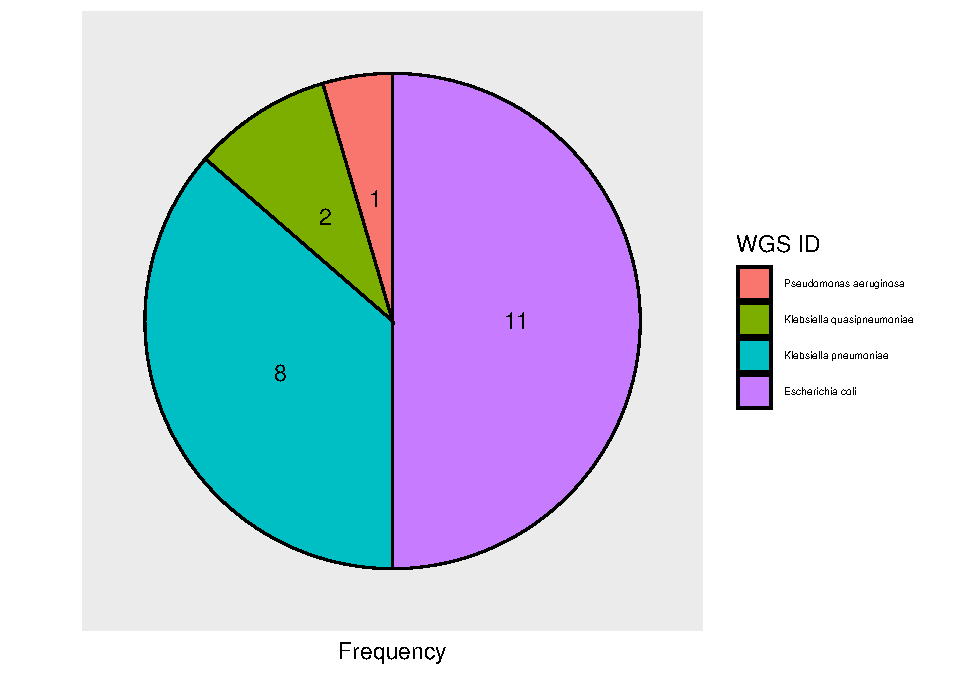
\includegraphics{qualifyr_report_2024-05-03_files/figure-latex/pie_chart-1.pdf}

\subsubsection{Result Classification}\label{result-classification}

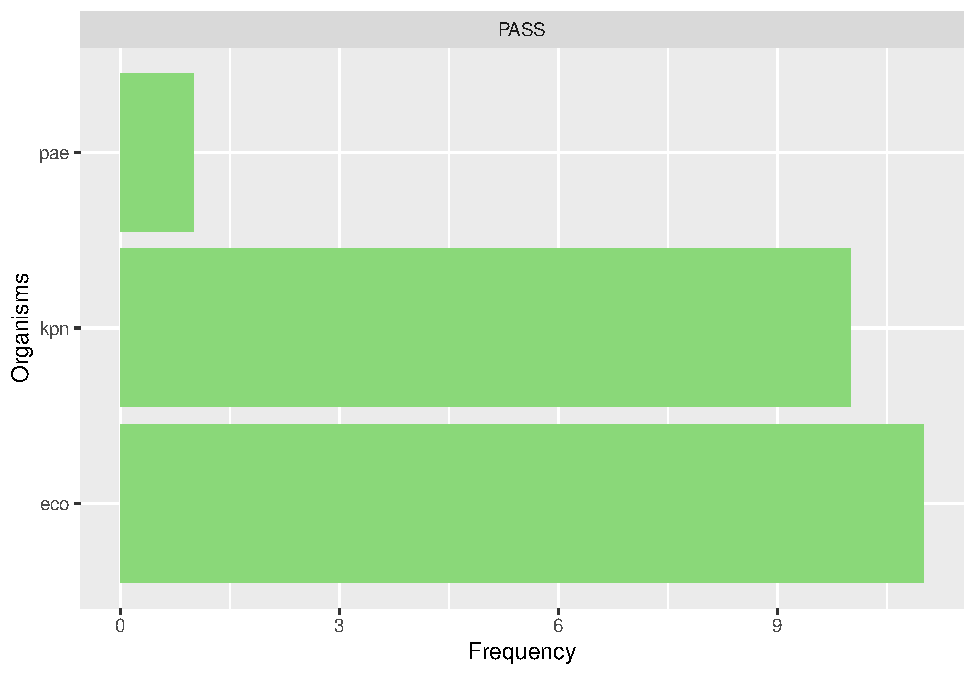
\includegraphics{qualifyr_report_2024-05-03_files/figure-latex/organism results-1.pdf}

\subsubsection{Number of contigs}\label{number-of-contigs}

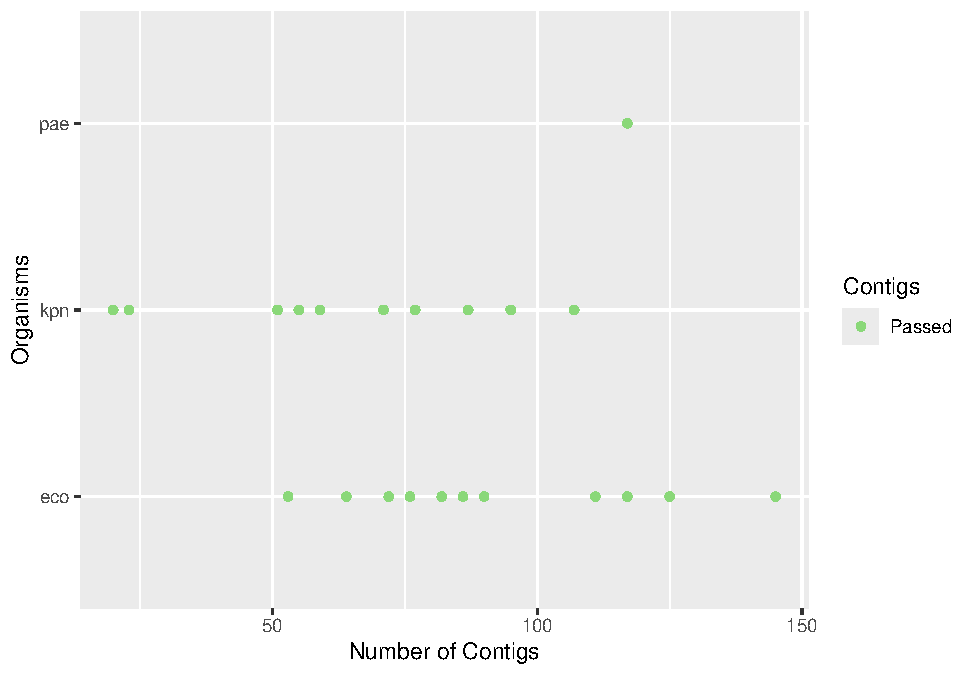
\includegraphics{qualifyr_report_2024-05-03_files/figure-latex/unnamed-chunk-1-1.pdf}

\subsubsection{N50 Value}\label{n50-value}

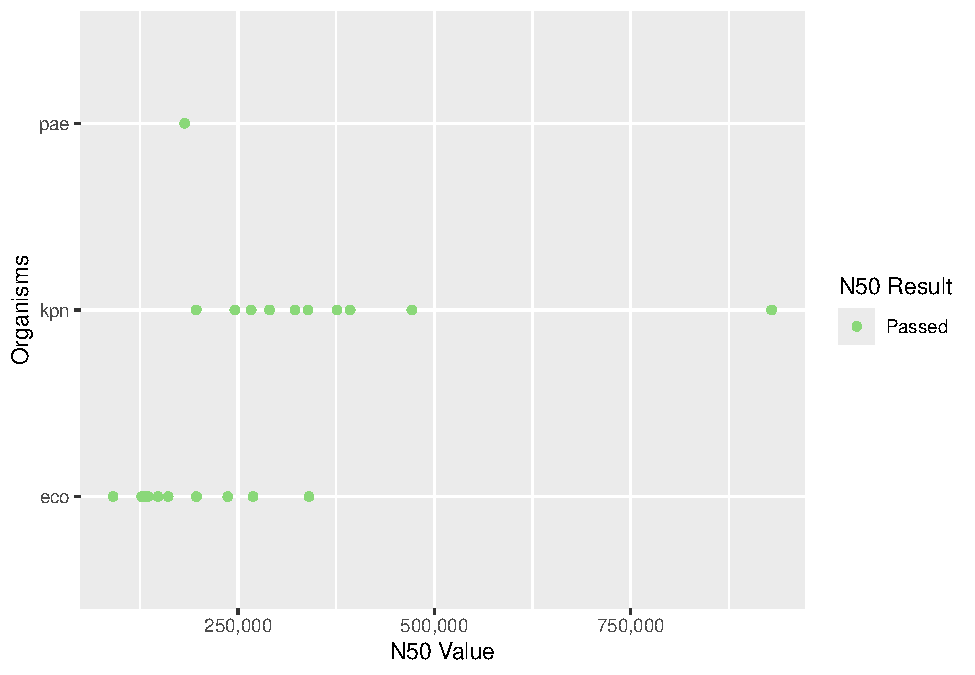
\includegraphics{qualifyr_report_2024-05-03_files/figure-latex/n50_result -1.pdf}

\subsubsection{Total Length}\label{total-length}

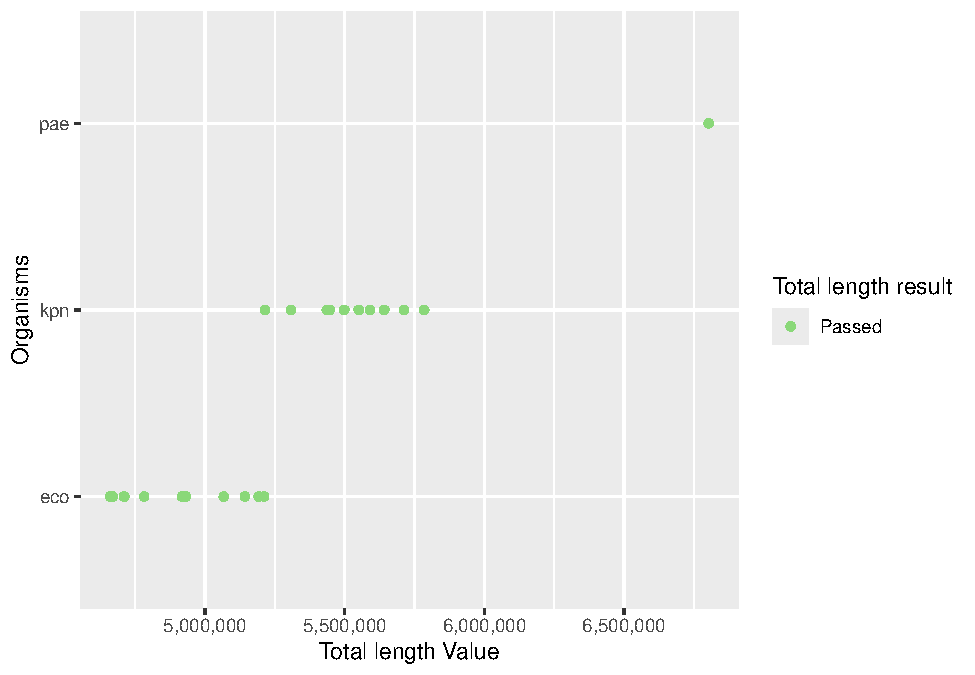
\includegraphics{qualifyr_report_2024-05-03_files/figure-latex/length_result -1.pdf}

\(\\\)

\subsubsection{RECOMMENDATION:}\label{recommendation}

\begin{longtable}[l]{>{\centering\arraybackslash}p{8cm}>{\centering\arraybackslash}p{3cm}>{\centering\arraybackslash}p{4cm}}
\toprule
\cellcolor[HTML]{D4D4D4}{\textbf{Sample ID}} & \cellcolor[HTML]{D4D4D4}{\textbf{Action}} & \cellcolor[HTML]{D4D4D4}{\textbf{Reason}}\\
\midrule
No further action required for this batch. &  & \\
\bottomrule
\end{longtable}

\end{document}
